\subsection{OB-5 (APS)}
Paměťová hierarchie se skrytou pamětí (cache memory), principy lokality a fungování skryté paměti. Architektura přímé, částečně asociativní, plně asociativní skryté paměti.

\subsubsection*{Paměťová hierarchie}

Rozdíl mezi rychlostí procesoru a rychlostí odpovědi paměti je velký (procesor vs DRAM --- 100x, procesor vs HDD --- 10 milionkrát).
Tento rozdíl se překlene paměťovou hierarchií.

\begin{itemize}
	\item L1 cache
	\begin{itemize}
		\item SRAM
		\item nejmenší, nejblíže jádru, díky tomu nejrychlejší
		\item velikost v řádu jednotek či desítek KB
		\item pro každé jádro zvlášť, bývá rozdělena na instrukční a datovou cache
		\item obsahuje právě nejpoužívanější data a instrukce
	\end{itemize}
	
	\item L2 cache
	\begin{itemize}
		\item SRAM
		\item větší, blízko jádra, latence větší než L1
		\item velikost v řádu stovek KB
		\item pro každé jádro zvlášť, společná pro instrukce a data
		\item obsahuje vše co je v L1 + druhá nejpoužívanější data a instrukce
	\end{itemize}
	
	\item L3 cache
	\begin{itemize}
		\item SRAM
		\item ještě větší, stále poměrně blízko jádrům, latence větší než L2
		\item velikost v řádu jednotek MB
		\item typicky sdílena více jádry, společná pro instrukce i data
		\item obsahuje vše co je v L2 + třetí nejpoužívanější data a instrukce
	\end{itemize}
	
	\item Hlavní paměť
	\begin{itemize}
		\item DRAM
		\item velká, mimo procesor, tedy latence zásadně vyšší než u cache
		\item velikost typicky v řádu jednotek či desítek GB, může být i větší/menší
		\item společná pro celý procesor(y), obsahuje data i instrukce
		\item obsahuje vše co je v L3 + naprostou většinu potřebných dat i instrukcí
	\end{itemize}
	
	\item Sekundární paměť
	\begin{itemize}
		\item HDD, SSD
		\item největší, nejpomalejší
		\item společná pro celý počítač, obsahuje vše
	\end{itemize}
	 
\end{itemize}

\subsubsection*{Principy lokality}
Programy typicky přistupují v daném okamžiku jen k malé části instrukčního a datového adresního prostoru.

\textbf{Časová lokalita:}
\begin{itemize}
	\item položky, ke kterým se přistupovalo nedávno, budou brzy zapotřebí znovu
	\item příklad: opakované procházení dat v cyklu, opakované čtení instrukcí v rekurzivních algoritmech
\end{itemize}

\textbf{Prostorová lokalita:}
\begin{itemize}
	\item položky poblíž právě používaných budou brzy zapotřebí také
	\item příklad: sekvenční přístup k instrukcím programu, sekvenční přístup k datovým polím nebo lokálním proměnným umístěným poblíž sebe
\end{itemize}

\subsubsection*{Principy fungování skryté paměti}
\begin{itemize}
	\item Cache block
	
	Souvislý, nedělitelný úsek hlavní paměti, který lze přenést do cache během jedné paměťové transakce.
	
	\item Cache hit
	
	Úspěšný přístup ke cache block --- tedy úspěšný přístup k datům/instrukcím, které jsou obsaženy v cache a jsou platné.
	
	\item Cache miss
	
	Opak cache hit --- neúspěšný přístup k datům/instrukcím v cache.
	
	\item Hit rate
	
	Úspěšnost přístupů do cache (poměr). 
	
	\item Miss rate
	
	Neúspěšnost přístupů do cache (poměr).
	
	\item Hit time
	
	Latence cache, čas na získání dat z dané úrovně cache.
	
	\item Miss penalty
	
	Celkový čas pro získání dat při výpadku (cache miss) dané úrovně (počítá se od dané úrovně dál).
\end{itemize}

Průměrný čas přístupu do paměti: Hit time + (Miss rate * Miss penalty)

\subsubsection*{Adresace skryté paměti}
Kusy hlavní paměti se do cache ukládají po blocích. Blok může být různě veliký, typicky obsahuje více bytů (nejmenších adreovatelných kusů paměti).


\begin{itemize}
	\item Přímo mapovaná cache
	\begin{itemize}
		\item každý set (řádek) cache obsahuje právě 1 blok.
		\item za sebou jdoucí bloky hlavní paměti se mapují do za sebou jdoucích bloků cache
		\item řádek = (Adresa v hlavní paměti / velikost bloku) \% počet řádků
		\item každý blok hlavní paměti má tedy vždy stejný blok cache kam se uloží.
		\item na stejný blok cache lze uložit více různých bloků paměti, musíme tedy uložit navíc číslo bloku hlavní paměti (část původní adresy) = Tag
	\end{itemize}
	
	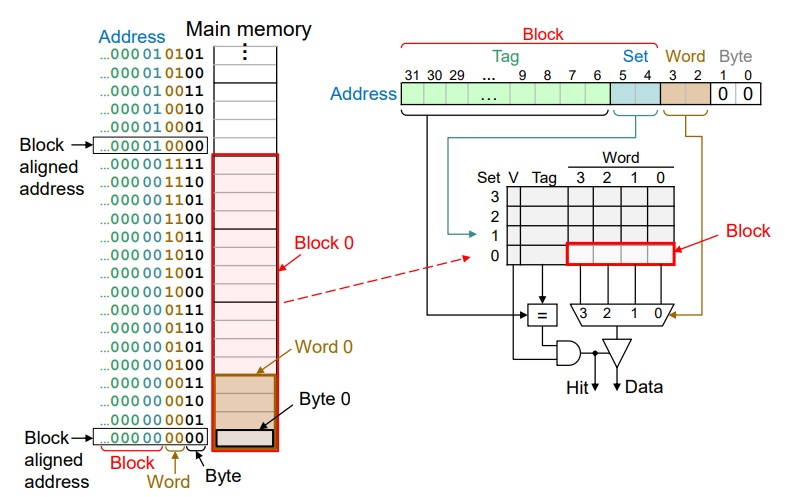
\includegraphics[width=0.8\textwidth]{img/OB-5_0.jpg}
	
	V takovéto cache ale často dochází ke kolizím, když chceme např. přistupovat do více různých částí hlavní paměti. Je ale snazší ji implementovat.
	
	\item Cache s částečným stupněm asociativity
	
	\begin{itemize}
		\item replikace instancí přímo mapované cache
		\item stupeň asociativity je počet takových instancí, neboli také počet cest v cache
		\item bloky hlavní paměti lze uložit na více různých míst (přesně na tolik, kolik je stupeň asociativity)
	\end{itemize}
	
	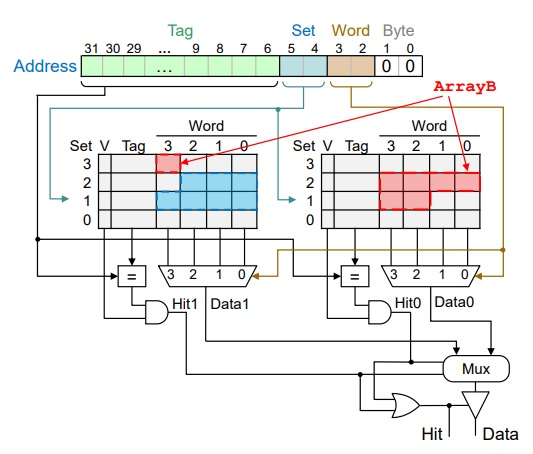
\includegraphics[width=0.7\textwidth]{img/OB-5_1.jpg}
	
	Vyšší složitost implementace, ale zásadně nižší miss rate.
	
	\item Plně asociativní cache
	\begin{itemize}
		\item počet cest je roven počtu bloků cache
		\item instance přímo mapované cache mají tedy jen jeden řádek (set)
		\item u každého bloku se ukládá celá jeho adresa v hlavní paměti
	\end{itemize}
	
	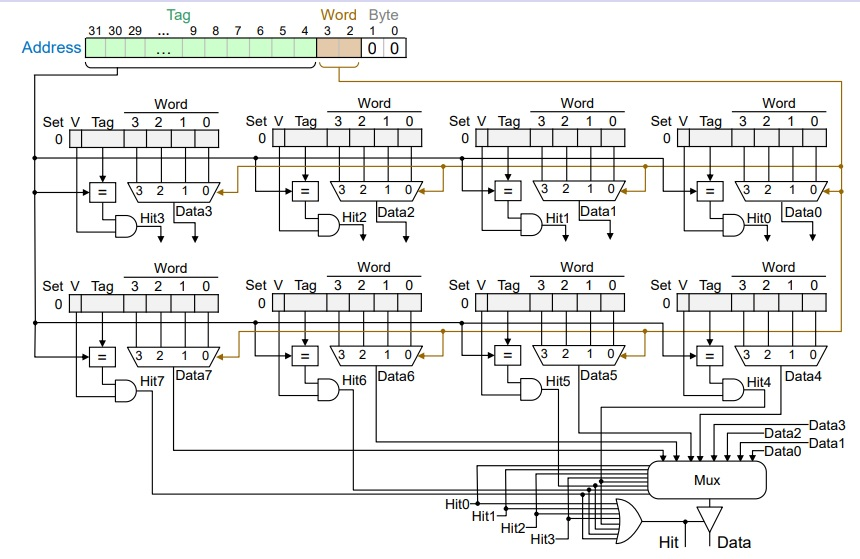
\includegraphics[width=0.75\textwidth]{img/OB-5_2.jpg}
	
	Nejnáročnější na HW prostředky, ale musí řešit maximální počet kolizí.
	
	
\end{itemize}